\documentclass{article}
\usepackage[utf8]{inputenc}
\usepackage{polski}
\usepackage{graphicx}
\usepackage{fancyhdr}
\usepackage{lastpage}
\usepackage{listings}

\pagestyle{fancy}

\fancyhf{}

\fancyfoot[C]{\thepage\ / \pageref{LastPage}} % Ustawienie numeracji stron w stopce

\fancypagestyle{plain}{ % Nadpisanie stylu strony tytułowej
    \fancyhf{}
    \renewcommand{\headrulewidth}{0pt} % Usunięcie nagłówka
    \fancyfoot[C]{\thepage\ / \pageref{LastPage}}
}

\title{Specyfikacja funkcjonalna projektu 1 w języku C}
\author{Miłosz Mertka i Sebastian Grosfeld}
\date{\today}

\begin{document}

\maketitle

\tableofcontents

\newpage

% Poniżej ustawiany jest nagłówek
\setlength{\headheight}{23pt}
\lhead{Miłosz Mertka\\Sebastian Grosfeld}
\rhead{Specyfikacja funkcjonalna\\projektu 1 w języku C}

\section{Wstęp teoretyczny}

Program porusza zagadnienia teorii grafów. Teoria grafów to dziedzina informatyki zajmująca się badaniem zjawisk przy wykorzystaniu grafów. Graf definiuje się następująco: $G=(V,E)$. $V$ jest zbiorem wierzchołków grafu, $E$ jest zbiorem jego krawędzi. \emph{Rysunek \ref{fig:graph}} pokazuje przykładowy graf.

\begin{figure}[htp]
    \centering
    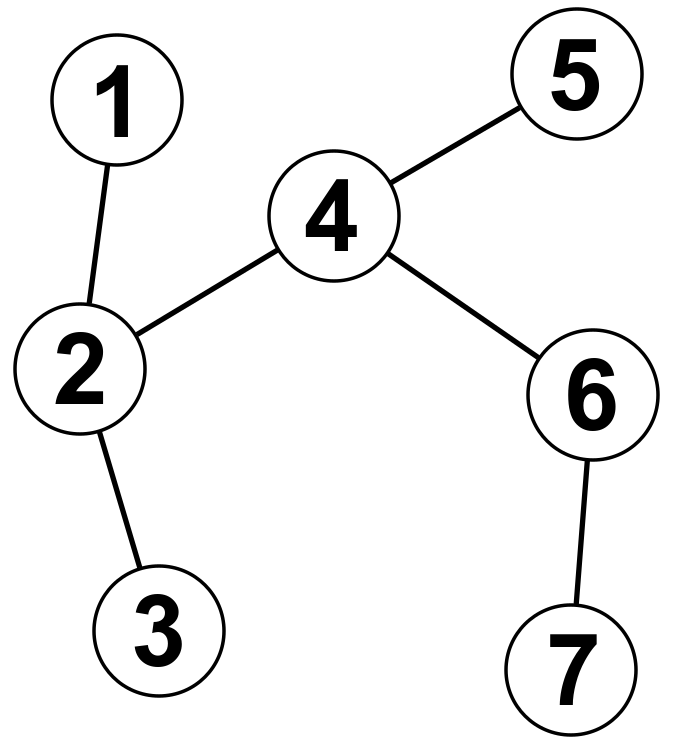
\includegraphics[width=5cm]{images/graph.png}
    \caption{Przykładowy graf}
    \label{fig:graph}
\end{figure}

Grafy można podzielić na \emph{nieskierowane} i \emph{skierowane}. Te pierwsze posiadają drogę zarówno z wierzchołka A do wierzchołka B, ale także z wierzchołka B do wierzchołka A. Grafy skierowane natomiast nie muszą posiadać zdefiniowanych przejść w obie strony dla danej pary wierzchołków A i B. W grafach skierowanych wierzchołki są ze sobą połączone łukami, które wskazują kierunek przejścia z jednego wierzchołka do drugiego (\emph{Rysunek \ref{fig:directed_graph}}).

\begin{figure}[htp]
    \centering
    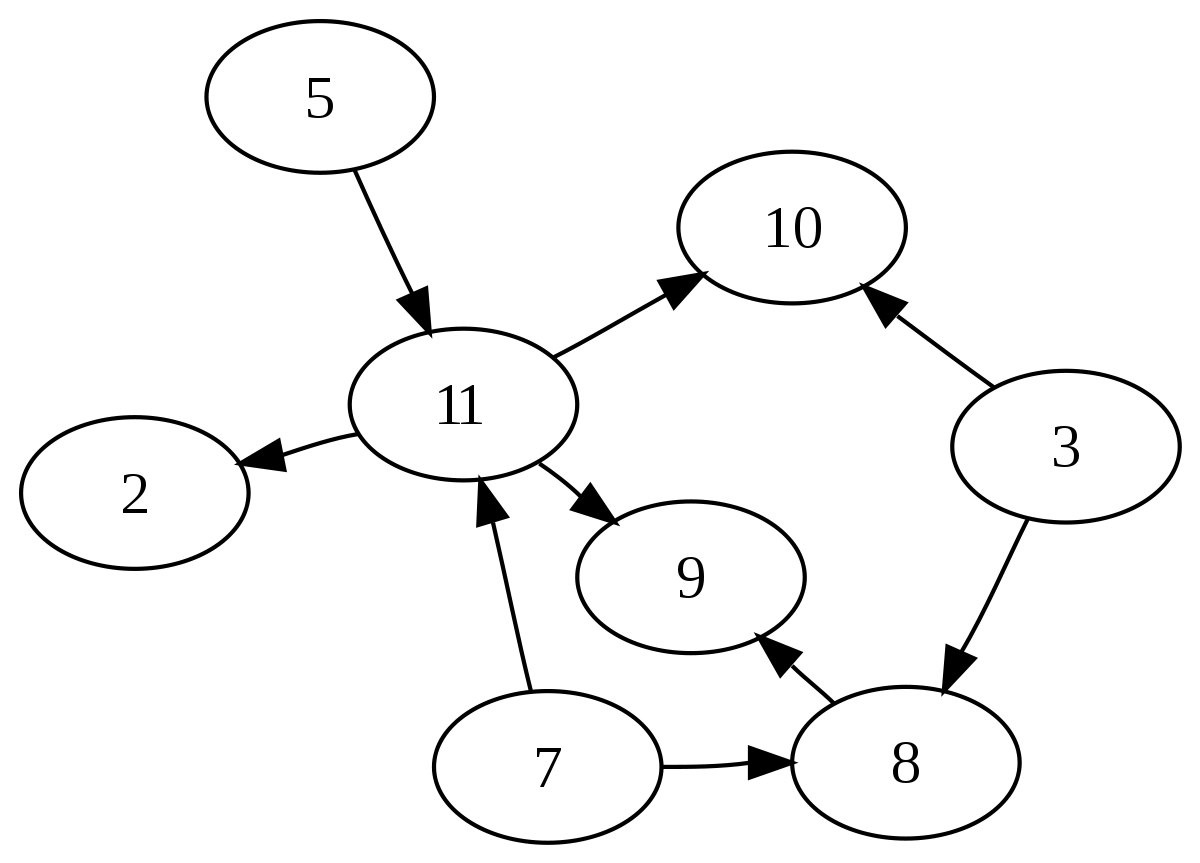
\includegraphics[width=7cm]{images/directed_graph.png}
    \caption{Przykładowy graf skierowany}
    \label{fig:directed_graph}
\end{figure}

\newpage
Krawędzie w grafach mogą również posiadać różne wagi. Taki graf nazywa się \emph{grafem ważonym}. Waga określa koszt przejścia z jednego wierzchołka do drugiego. Przykładowy graf ważony przedstawia \emph{Rysunek \ref{fig:weight_graph}}. W przypadku grafu skierowanego można zdefiniować różne wagi dla dwóch łuków łączących tą samą parę wierchołków.

\begin{figure}[htp]
    \centering
    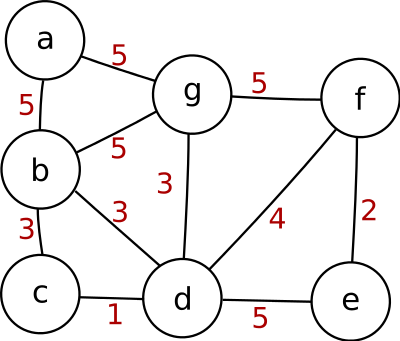
\includegraphics[width=6cm]{images/graph_weights.png}
    \caption{Przykładowy graf nieskierowany ważony}
    \label{fig:weight_graph}
\end{figure}

Grafy bada się pod kątem ich \emph{spójności}. Graf jest spójny, jeśli zawsze istnieje droga między dowolnymi wierzchołkami grafu. Do badania spójności grafu można wykorzystać znane algorytmy przeszukiwania grafu. \emph{Rysunek \ref{fig:inconsistent_graph}} pokazuje przykładowy graf niespójny.

\begin{figure}[htp]
    \centering
    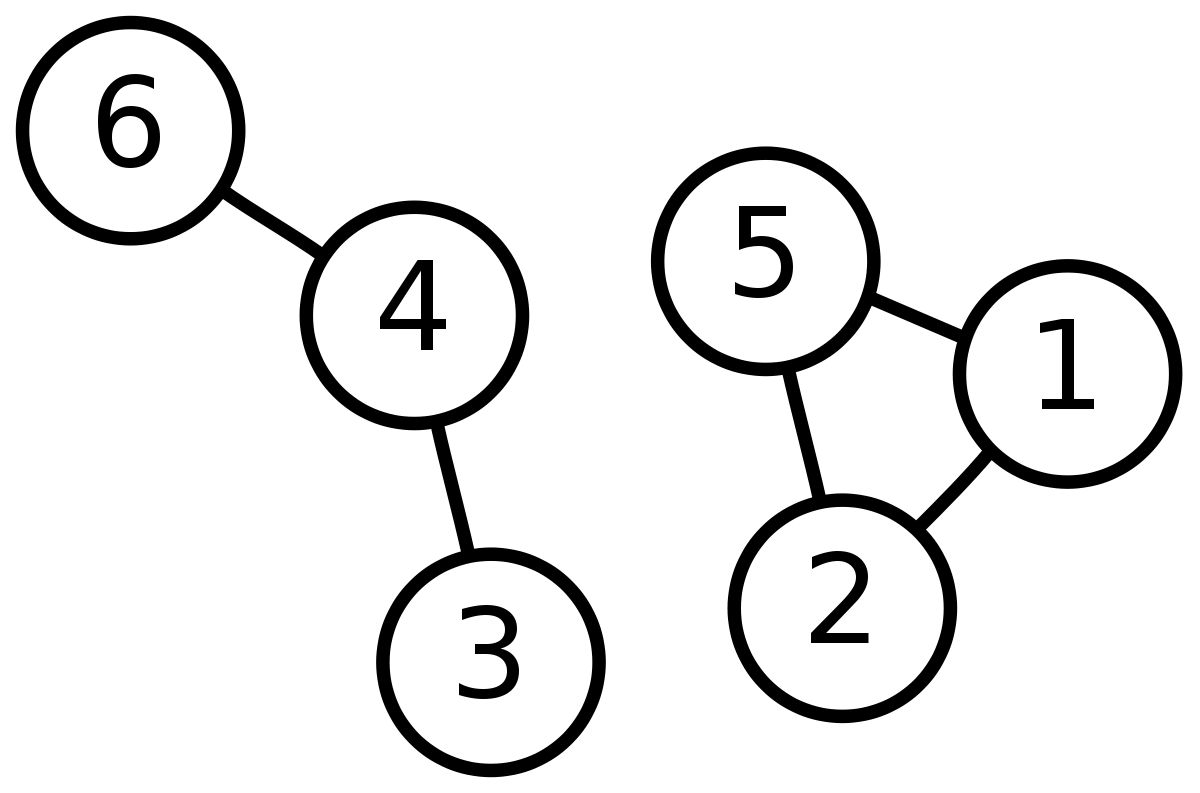
\includegraphics[width=5cm]{images/graph_inconsistent.png}
    \caption{Przykładowy graf niespójny}
    \label{fig:inconsistent_graph}
\end{figure}

Grafy posiadają praktyczne zastosowanie między innymi w systemach nawigacji drogowej. Tutaj za wierzchołki grafu można potraktować kolejne skrzyżowania, krawędzie to drogi łączące te skrzyżowania, a waga to koszt przejazdu od jednego skrzyżowania do drugiego. W ten sposób można następnie zastosować znane algorytmy szukania optymalnej drogi w grafie między zadanymi wierzchołkami. W wyniku tego można otrzymać w nawigacji samochodowej optymalną trasę dojazdu do zadanego celu.

\section{Cel projektu}
Celem projektu jest stworzenie programu, który będzie w stanie wykonać następujące zadania:
\begin{enumerate}
    \item Wygeneruje graf w postaci siatki (\emph{Rysunek \ref{fig:graf_pp}}) o podanej ilości kolumn i wierszy, wierzchołki i wagi krawędzi losowane w podanym zakresie wartości.
    \item Zapisze taki graf do pliku o ustalonym formacie.
    \item Przeczyta z pliku o ustalonym formacie taki graf.
    \item Potrafi określić czy dany graf jest spójny za pomocą algorytmu BFS.
    \item Potrafi wyznaczyć w tym grafie najkrótsze ścieżki pomiędzy wybranymi parami wierzchołków, korzystając z algorytmu Dijkstry.
\end{enumerate}

\begin{figure}[htp]
        \centering
        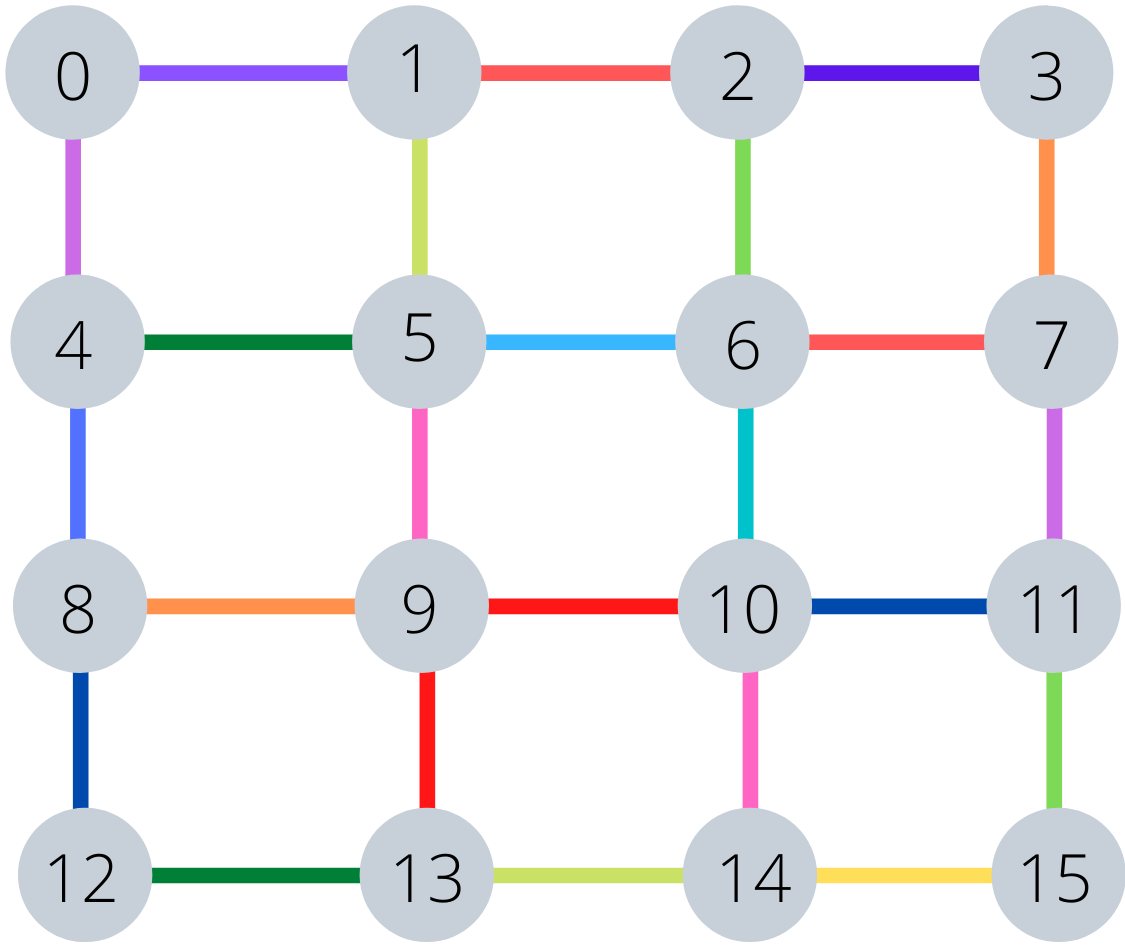
\includegraphics[width=5cm]{images/graf_pp.png}
        \caption{Wizualizacja przykładowego, wygenerowanego grafu}
        \label{fig:graf_pp}
\end{figure}

\newpage

\section{Uruchamianie programu}
Program działa w środowisku konsolowym. W celu jego uruchomienia należey wywołać odpowiednią komendę w konsoli. Należy przejść do katalogu w którym znajduje się program i wywołać go używając jego nazwy pliku. W trakcie wywoływania programu należy przekazać do niego także odpowiednie argumenty.

\subsection{Argumenty wywołania}
Możliwe do przekazania argumenty:
\begin{itemize}
    \item \emph{tryb\textunderscore działania} -- określa, co program ma wykonać. W zależności od wybranego trybu działania należy także przekazać inne argumenty do programu. Możliwe są następujące tryby działania programu:
    \begin{itemize}
        \item \textbf{generate\textunderscore wages} -- generuje graf ze wszystkimi krawędziami i przypisuje do nich losowe wagi w zadanym jako argumenty zakresie
        \item \textbf{generate\textunderscore consistent} -- generuje graf spójny
        \item \textbf{generate\textunderscore random} -- generuje graf z losowymi wagami i krawędziami (\textit{nie ma gwarancji spójności grafu})
        \item \textbf{analyze} -- analizuje graf wczytany z pliku pod kątem spójności i opcjonalnie wyświetla najkrótszą drogę między zadanymi wierzchołkami
    \end{itemize}
    \item \emph{nazwa\textunderscore pliku} -- określa plik, do którego graf ma zostać zapisany po wygenerowaniu. W przypadku trybu \textbf{analyze} jest to plik z definicją grafu, który ma zostać wczytany do programu
    \item \emph{liczba\textunderscore wierszy} -- liczba wierszy grafu do wygenerowania (liczba naturalna większa od zera)
    \item \emph{liczba\textunderscore kolumn} -- liczba kolumn grafu do wygenerowania (liczba naturalna większa od zera)
    \item \emph{waga\textunderscore od} -- minimalna wartość do wylosowania dla wagi (liczba rzeczywista nieujemna)
    \item \emph{waga\textunderscore do} -- maksymalna wartość do wylosowania dla wagi (liczba rzeczywista nieujemna)
    \item \emph{droga\textunderscore źródło} -- numer węzła startowego dla szukania ścieżki
    \item \emph{droga\textunderscore cel} -- numer węzła docelowego dla szukania ścieżki
\end{itemize}

\newpage

\subsection{Schemat wywołania}
Program należy wywołać z odpowiednimi argumentami w zależności od wybranego trybu pracy.

\subsubsection{Tryb generate\textunderscore wages}
Składnia:\\
\textit{nazwa\textunderscore programu tryb\textunderscore działania nazwa\textunderscore pliku liczba\textunderscore wierszy liczba\textunderscore kolumn waga\textunderscore od waga\textunderscore do}

\medskip

\noindent Przykład:\\
\textit{./grapher generate\textunderscore wages graf.txt 8 5 1 3}\\
Wywołanie powyższego polecenia spowoduje wygenerowanie grafu ze wszystkimi krawędziami o losowych wagach. Wagi są losowane z przedziału $<1, 3>$. Wygenerowane zostanie 8 wierszy i 5 kolumn. Wynikowy graf zostanie zapisany do pliku \emph{graf.txt}.

\subsubsection{Tryb generate\textunderscore consistent}
Składnia:\\
\textit{nazwa\textunderscore programu tryb\textunderscore działania nazwa\textunderscore pliku liczba\textunderscore wierszy liczba\textunderscore kolumn}

\medskip

\noindent Przykład:\\
\textit{./grapher generate\textunderscore consistent graf.txt 7 6}\\
Wywołanie powyższego polecenia spowoduje wygenerowanie grafu spójnego. Wygenerowane zostanie 7 wierszy i 6 kolumn. Wynikowy graf zostanie zapisany do pliku \emph{graf.txt}.

\subsubsection{Tryb generate\textunderscore random}
Składnia:\\
\textit{nazwa\textunderscore programu tryb\textunderscore działania nazwa\textunderscore pliku liczba\textunderscore wierszy liczba\textunderscore kolumn waga\textunderscore od waga\textunderscore do}

\medskip

\noindent Przykład:\\
\textit{./grapher generate\textunderscore random graf.txt 12 15 2 8}\\
Wywołanie powyższego polecenia spowoduje wygenerowanie grafu o losowych wagach i krawędziach (\emph{brak gwarancji spójności grafu}). Wagi są losowane z przedziału $<2, 8>$. Wygenerowane zostanie 12 wierszy i 15 kolumn. Wynikowy graf zostanie zapisany do pliku \emph{graf.txt}.

\newpage

\subsubsection{Tryb analyze}
Składnia:\\
\textit{nazwa\textunderscore programu tryb\textunderscore działania nazwa\textunderscore pliku  [droga\textunderscore źródło] [droga\textunderscore cel] [droga\textunderscore źródło(1)] [droga\textunderscore cel(1)]}

\medskip

\noindent Przykład:\\
\textit{./grapher analyze graf.txt 16 8}\\
Wywołanie powyższego polecenia spowoduje analizę grafu z pliku \emph{graf.txt} pod kątem jego spójności. Dodatkowo program spróbuje znaleźć najkrótszą ścieżkę od wierzchołka 16 do wierzchołka 8.
\section{Scenariusze uruchomienia i wyniki}
\subsection{Przykładowe scenariusze wraz z wynikami}
Wywołuję program dla następujących parametrów.
\begin{itemize}
\item\textit{./grapher generate\textunderscore random graf.txt 7 4 0 1 2 7}

\medskip

Po wywołaniu tego polecenia program zapisuje wygenerowany graf do pliku \emph{graf.txt}, a jeśli taki nie istnieje to go utworzy. Wypisuje się komunikat: 

\medskip

\textit{consistent}\\
$(2,7): 2(0,3) \rightarrow 3(0,7) \rightarrow 7$

\medskip

Program informuje, że wygenerowany graf jest spójny oraz, że została wyznaczona najkrótsza ścieżka z wierzchołka 2 do wierzchołka 7 biegnąca przez wierzchołek 3 i waga krawędzi między wierzchołkami 2 i 3 wynosi 0,3 , a między wierzchołkami 3 i 7 wynosi 0,7.
\item \textit{./grapher analyze graf.txt 2 7 12 15}

\medskip

Program odczytuje z pliku \emph{graf.txt} o ustalonym formacie graf, określa jego spójność i wyznacza najkrótsze ścieżki między podanymi parami wierzchołków i wypisuje komunikat:

\medskip

\textit{inconsistent}\\
$(2,7): 2(0,3) \rightarrow 3(0,7) \rightarrow 7$\\
\textit{(12,15): The path does not exist}

\medskip

Program informuje, że odczytany graf jest niespójny. Wypisuje też informacje o najkrótszej ścieżce z wierzchołka 2 do 7 tak jak w poprzednim przykładzie. Pojawia się komunikat o tym, że ścieżka między wierzchołkiem 12 i 15 nie istnieje.

\item \textit{./grapher generate\textunderscore consistent graf.txt 7 4}

\medskip

Program generuje graf spójny mający 7 wierszy i 4 kolumny oraz zapisuje go do pliku \emph{graf.txt} w ustalonym formacie.
\end{itemize}
\subsection{Format pliku do zapisu i odczytu}
W pierwszej linii pliku znajduje się kolejno liczba wierszy, a następnie po spacji liczba kolumn w grafie. Następne linie zawierają informacje o kolejnych wierzchołkach, czyli druga linia zawiera informacje o wierzchołku 0 trzecia o 1 itd. W linii są wypisane numery wierchołków sąsiadujących, a po znaku ':' waga krawędzi łącząca wierzchołek z jego sąsiadem.

\medskip

\noindent Przykład pliku:
\begin{lstlisting}
7 4
    1 :0.8864  4 :0.2187
    5 :0.2465  2 :0.6445  0 :0.4630 
    6 :0.8650  3 :0.4293  1 :0.6024
    7 :0.5702  2 :0.8645 
    8 :0.9452  0 :0.8963  5 :0.9299 
    1 :0.5950  9 :0.3164  6 :0.4032 4 :0.4428 
    10 :0.7910  7 :0.7013  2 :0.2005  5 :0.3551
    6 :0.9338  3 :0.7970  11 :0.7191 
    4 :0.7500  12 :0.5486  9 :0.2541 
    13 :0.8647  5 :0.8896  8 :0.4952  10 :0.4018 
    14 :0.5676  6 :0.5809  9 :0.7797  11 :0.3769
    15 :0.3166  10 :0.1481  7 :0.8363 
    13 :0.5380  16 :0.8456  8 :0.5238
    17 :0.5984  9 :0.7875  12 :0.7383  14 :0.4574
    10 :0.8801  15 :0.6167  18 :0.2663  13 :0.2256
    19 :0.9069  11 :0.7381  14 :0.5723
    20 :0.1541  17 :0.3985  12 :0.2946
    21 :0.7576  13 :0.4858  16 :0.6456  18 :0.6265
    17 :0.6628  22 :0.9203  14 :0.8394  19 :0.2751
    18 :0.6976  15 :0.4893  23 :0.5604
    24 :0.8901  21 :0.5619  16 :0.3583 
    17 :0.8437  20 :0.3316  25 :0.7968  22 :0.9281
    21 :0.6354  23 :0.3344  18 :0.4302  26 :0.3746
    27 :0.8914  22 :0.8708  19 :0.4478
    20 :0.3517  25 :0.2054
    21 :0.6830  24 :0.3148  26 :0.5449
    27 :0.2105  22 :0.8159  25 :0.4989
    26 :0.4427  23 :0.4355
\end{lstlisting}
Przykładowo w pliku powyżej wierzchołek 0 sąsiaduje z wierzchołkiem 1 i krawędź od 0 do 1 ma wagę 0.8864 oraz sąsiaduje z wierzchołkiem 4 i krawędź od 0 do 4 ma wagę 0.2187.
\section{Komunikaty błędów}

W razie napotkania błędu program przerywa działanie i wyświetla stosowny komunikat dla danego błędu.

\medskip

\noindent Program może wyświetlić następujące komunikaty:
\begin{itemize}
    \item \textbf{Allocation error} -- podczas działania programu nie udało się zaalokować miejsca w pamięci. Zazwyczaj jest to związane z brakiem dostępnej wolnej pamięci operacyjnej.
    \item \textbf{File stream error} -- nie udało się otworzyć pliku do odczytu lub zapisu.
    \item \textbf{Invalid number of arguments} -- przekazano za mało lub za dużo argumentów.
    \item \textbf{Invalid mode} -- nieprawidłowy tryb działania programu (argument \emph{tryb\textunderscore działania} posiada nieprawidłową wartość).
    \item \textbf{Invalid arguments} -- podane argumenty są błędne (na przykład podano liczby ujemne dla określenia liczby wierszy i kolumn).
\end{itemize}

\end{document}
